%%%%%%%%%%%%%%%%%%%%%%%%%%%%%%%%%%%%%%%%%%%%%%%%%%%%%%%%%%%%%%%%%%%%%%%
%% Related Work
\subsection{Aufbau}
\label{sec:basic-aufbau}
    
Dieses Kapitel befasst sich mit dem Aufbau der Versuchsanlage und der verwendeten Hardware. Dabei werden die Aspekte des räumlichen Aufbau genauso betrachtet wie die Netzwerkinfrastruktur und die genutzten Roboter und Sensoren.



\subsubsection{Aufbau Teststand}

 \begin{figure}[h]
 	\centering
 	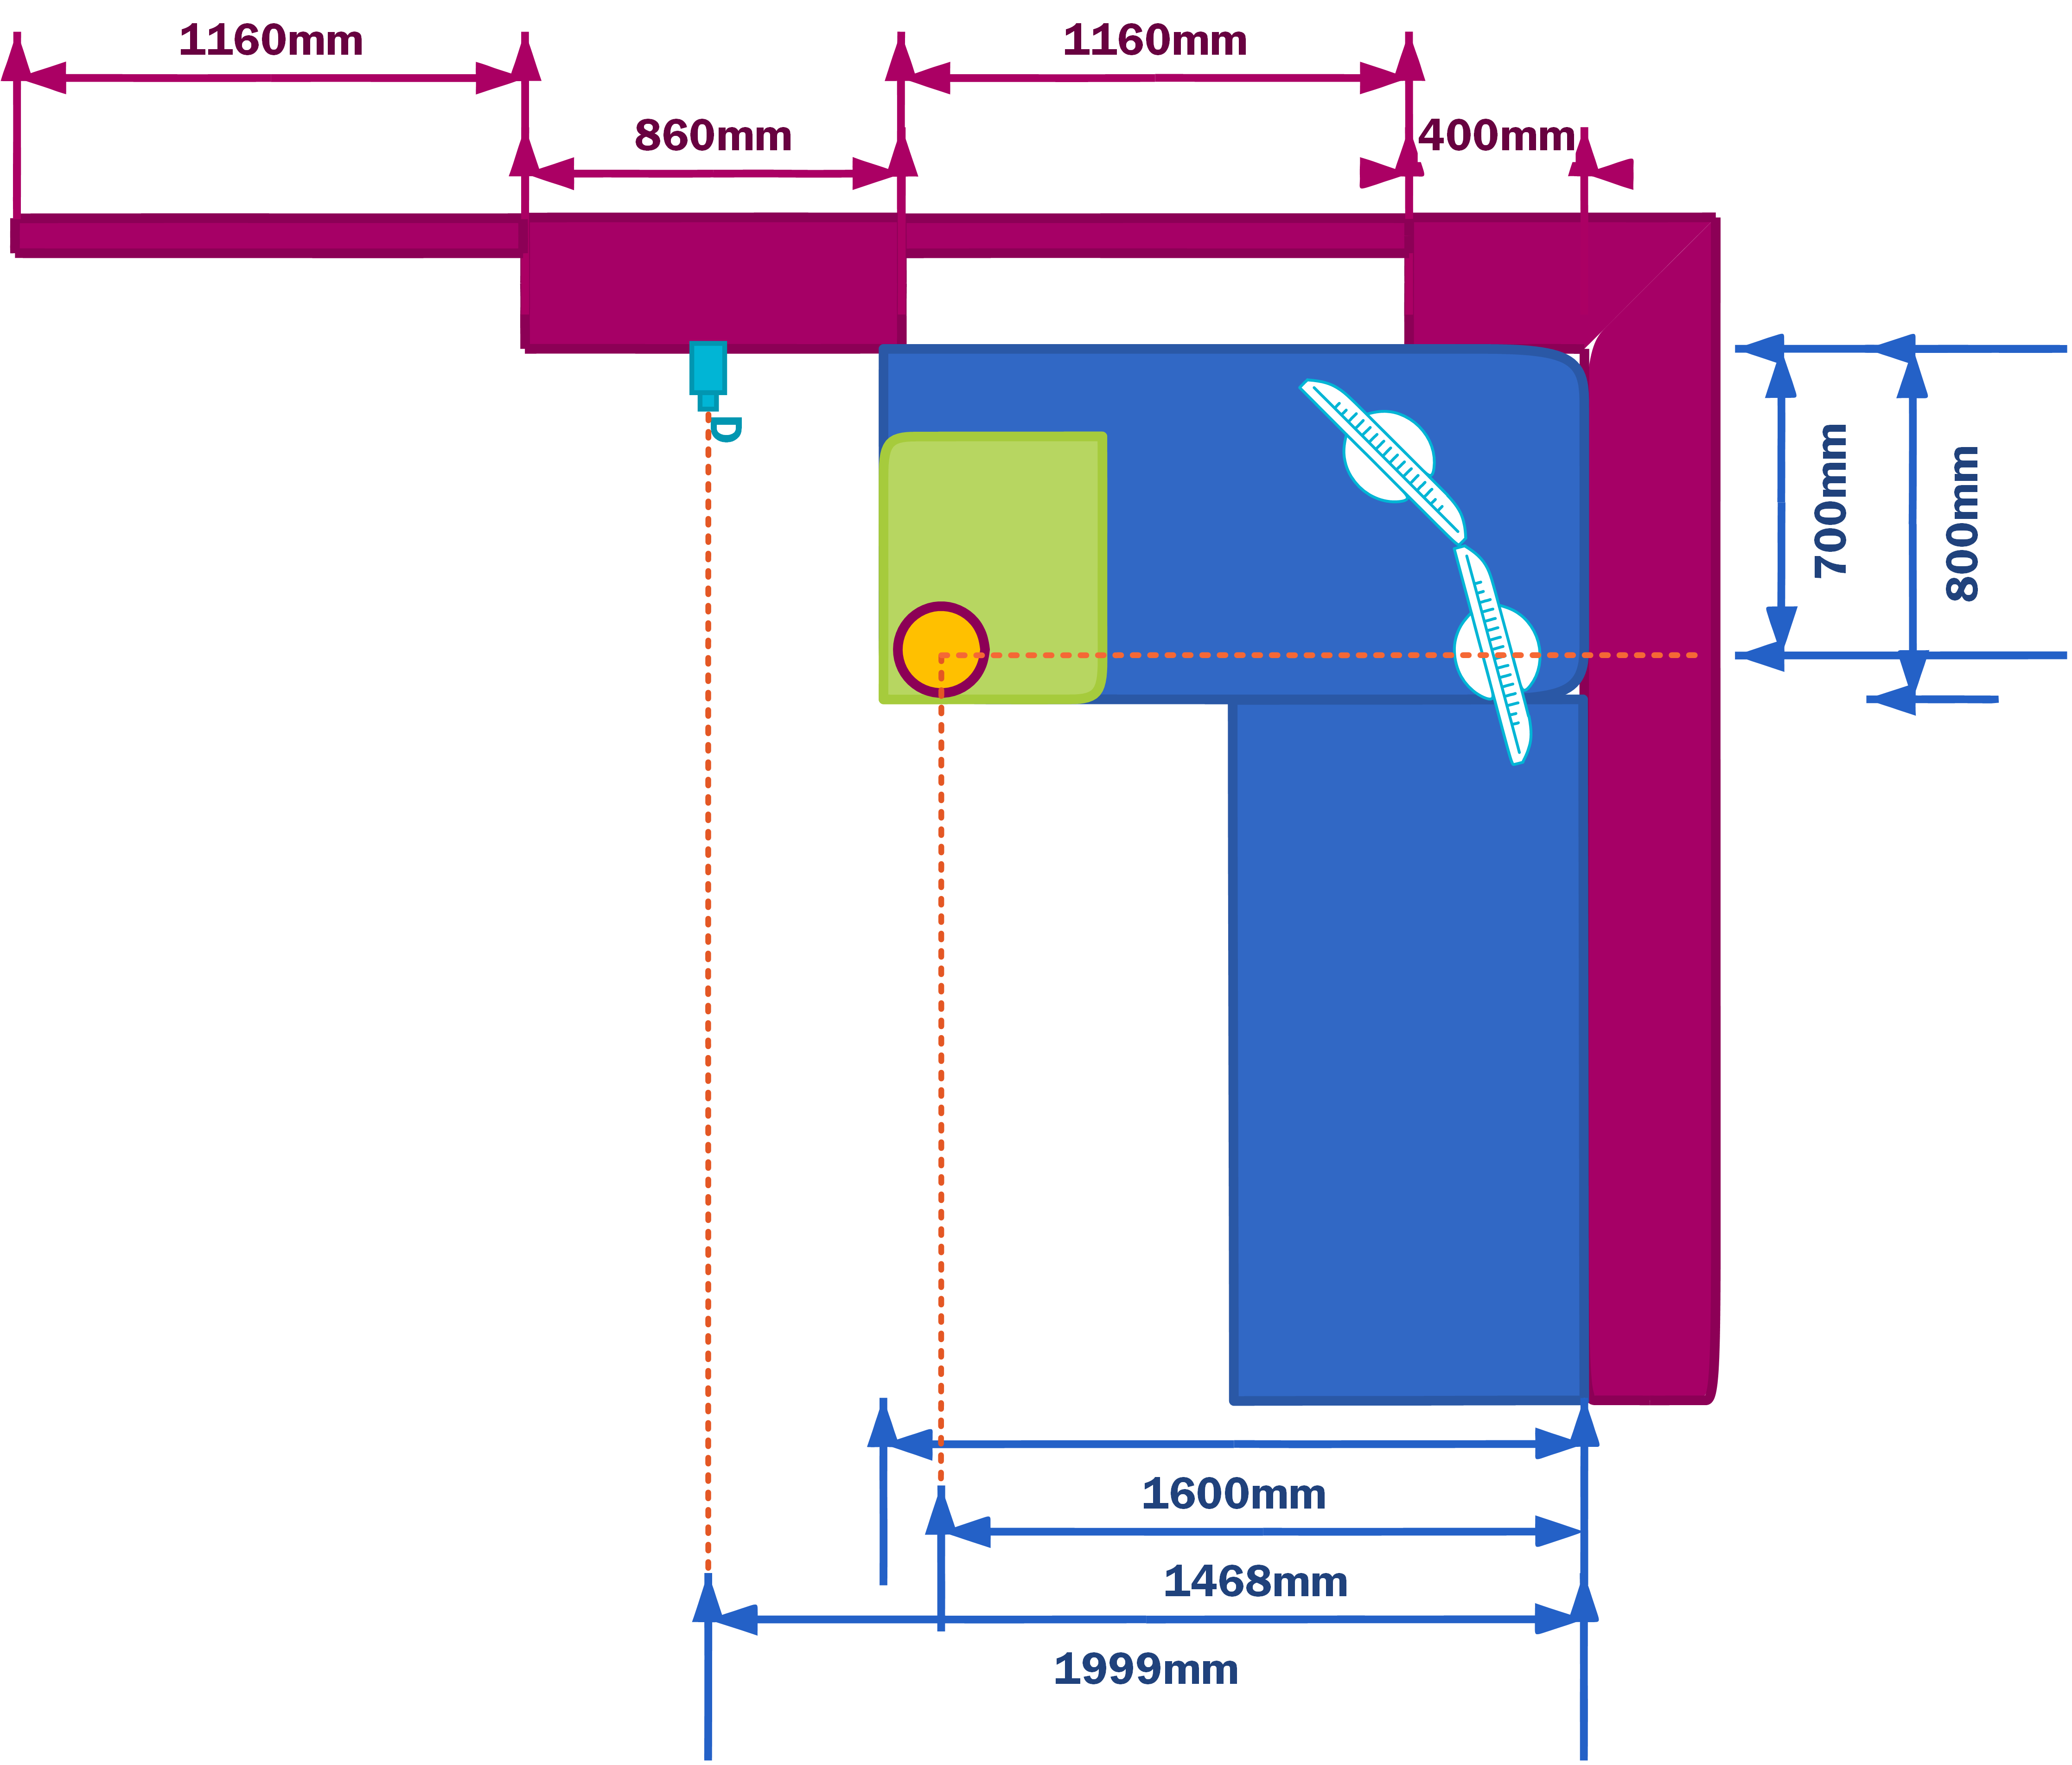
\includegraphics[scale=0.8]{fig/ZeichnungRaum}   
 	\caption[Aufbau Teststand: Draufsicht]{Der Aufbau}
 	\label{fig:basic-aufbau-teststand}
 \end{figure}
 
 
  \begin{figure}[h]
  	\centering
  	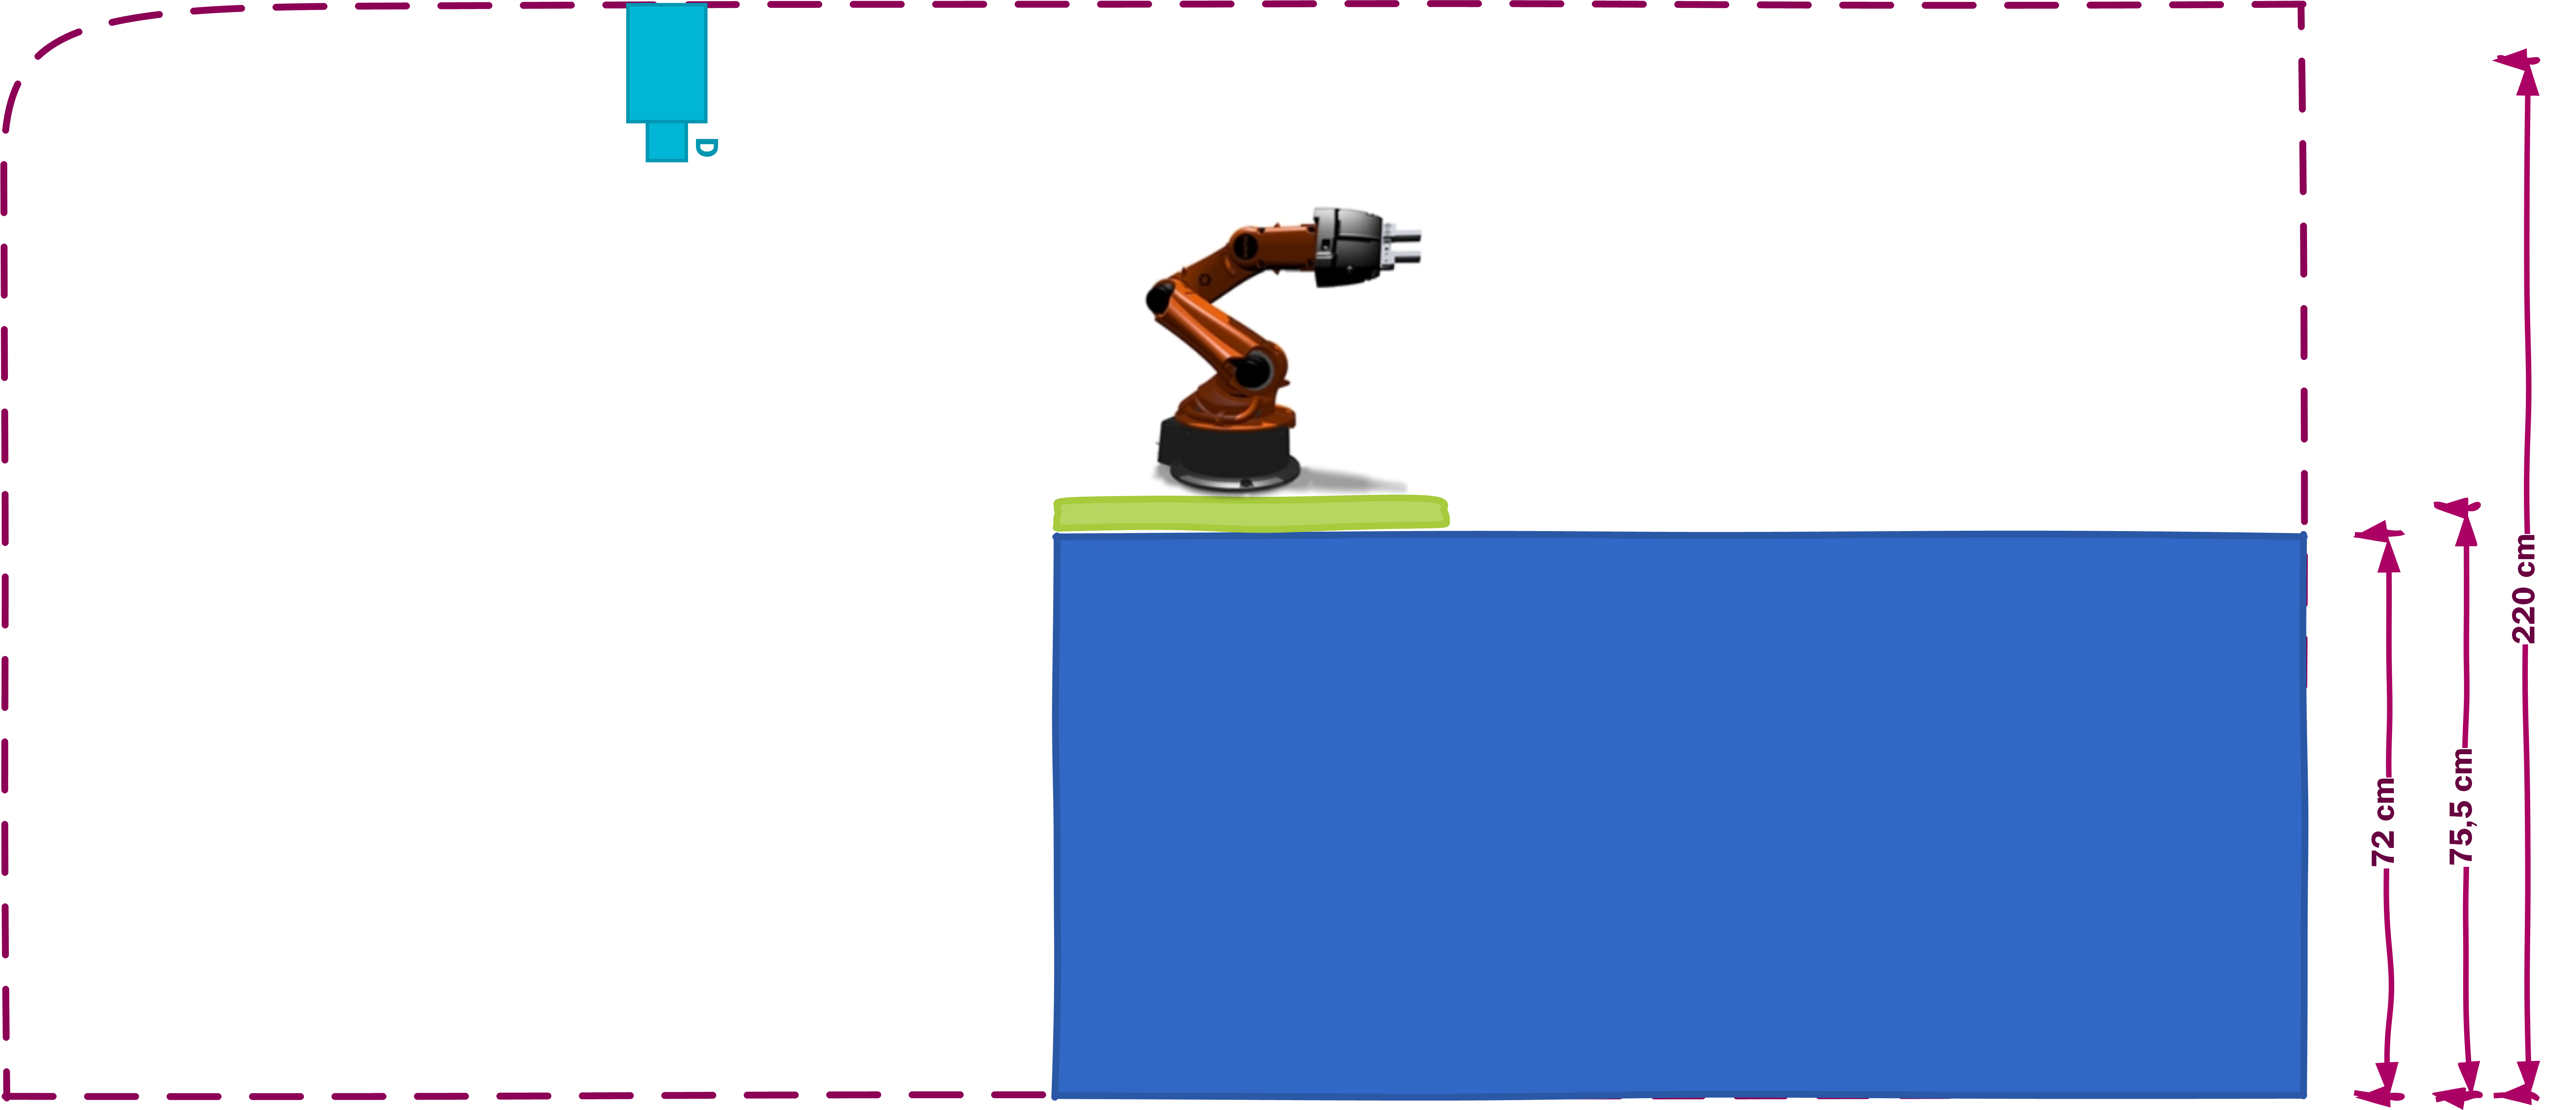
\includegraphics[scale=0.5]{fig/ZeichnungRaumH}   
  	\caption[Aufbau Teststand: Draufsicht]{Der Aufbau}
  	\label{fig:basic-aufbau-teststand}
  \end{figure}
